\section{Introduction}

Let $\mathbb{Z}^d$ be the $d$-dimensional integer lattice graph.
Given a subset $R \subseteq \mathbb{Z}^d$, we define a \emph{domino tiling} of $R$ to be a partition of the subset into disjoint adjacent pairs; in other words, it is a perfect matching of the subgraph induced by $R$.
In this note, we determine whether or not certain subsets of the lattice admit tilings which do not include specified substructures.
If $T$ is a domino tiling of a subset $R \subseteq \mathbb{Z}^d$ and $D$ is a collection of dominoes, we say that $T$ contains a \emph{substructure isomorphic to $D$} if there is a graph isomorphism $\phi \colon \mathbb{Z}^d \to \mathbb{Z}^d$ such that $\phi(\delta) \in T$ for each $\delta \in D$. A basic form of this question to consider is that for a square grid and the \say{pair} configuration
\begin{equation}
  D_\mathrm{pair} = \Big\{\{(0, 0), (1, 0)\}, \{(0, 1), (1, 1)\}\Big\}. 
\end{equation}
It is not difficult to see that every tiling of the grid must contain a pair.
Indeed, if a pair-free tiling $T$ exists, we may assume, without loss of generality, that it contains the domino labeled $1$ in Figure \ref{fig:impossible-grid}.
It follows that $T$ must also contain the domino labeled $2$, and from there the one labeled $3$, and so on. 
Eventually, this process forces a pair to be formed after the $(2n - 2)$th domino is placed, yielding a contradiction. 

\begin{figure}[h]
  \centering
  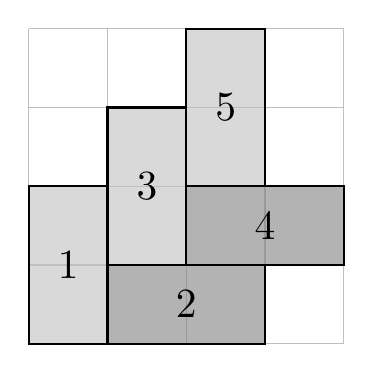
\begin{tikzpicture}[every node/.style={scale=1.5}]
    \draw[step=1cm, black!25] (0,0) grid (4,4);

    \draw[fill=black!25, fill opacity=0.6, thick] (0, 0) rectangle (1, 2);
    \draw[fill=black!50, fill opacity=0.6, thick] (1, 0) rectangle (3, 1);
    \draw[fill=black!25, fill opacity=0.6, thick] (1, 1) rectangle (2, 3);
    \draw[fill=black!50, fill opacity=0.6, thick] (2, 1) rectangle (4, 2);
    \draw[fill=black!25, fill opacity=0.6, thick] (2, 2) rectangle (3, 4);

    \node at (0.5, 1) {$1$};
    \node at (2, 0.5) {$2$};
    \node at (1.5, 2) {$3$};
    \node at (3, 1.5) {$4$};
    \node at (2.5, 3) {$5$};
  \end{tikzpicture}
  \caption{The impossibility of constructing of pair-free tiling of a $4 \times 4$ grid.}\label{fig:impossible-grid}
\end{figure}

The theory of domino tilings has been well-studied (see \cite{saldanha1995}), and is occasionally described in terms of tiling subsets of $\mathbb{R}^2$ with sets congruent to a $1 \times 2$ closed rectangle while allowing boundaries to overlap. 
Notably, it was proven by Thurston in \cite{thurston1990} that every simply connected region $\Omega \subseteq \mathbb{R}^2$ is \emph{flip-connected}, in the sense that any two tilings can be obtained from one another by repeatedly locating a pair (in this setting, two dominoes forming a $2 \times 2$ square) and performing a $90^\circ$ rotation.
In particular, if a tiling of a simply connected region $\Omega$ does not contain a pair, then it must be the 
\emph{only} tiling that $\Omega$ admits.
A general method for counting the number of domino tilings of a planar region due to P.~W.~Kasteleyn is given in \cite{kasteleyn1961} and a generalization to bipartite graphs may be found in \cite{lieb1993}.
For example, for an $n \times n$ grid where $n$ is even, the number of tilings is given by
\begin{equation}
  \prod_{j = 1}^{n/2} \prod_{k = 1}^{n/2} \left[ 4 \cos\left(\frac{j\pi}{n+1}\right)\!{\rule{0pt}{12pt}}^2 + 4\cos\left(\frac{k\pi}{n+1}\right)\!{\rule{0pt}{12pt}}^2 \!{\rule{0pt}{18pt}}\, \right].
\end{equation}
In principle, methods such as these may be used to show non-uniqueness of tilings. However, to the best of the author's knowledge, this approach does not appear in the literature.


The main result of this paper resolves the pair-free tiling problem for a special class of subsets $R \subseteq \mathbb{Z}^2$ analogous to compact $2$-manifolds in the plane. 
In Section \ref{sec:basics}, we develop basic notions and results for these subsets.
In Section \ref{sec:main}, we prove the main result via an argument reminiscent of the divergence theorem, equating the sum of a quantity over the region $R$ with the sum of another quantity over the \say{boundary} of $R$.
Finally, we apply the same type of argument in $\mathbb{Z}^3$ to obtain a similar result for grid graphs in Section \ref{sec:three-dimensions}.
